\documentclass[11pt]{article}
\usepackage{geometry}                
\geometry{letterpaper}                   

\usepackage{graphicx}
\usepackage{amssymb}
\usepackage{epstopdf}
\usepackage{natbib}
\usepackage{amssymb, amsmath}
\usepackage{color}
\usepackage{listings}
\lstloadlanguages{Matlab} 

\lstset{ %
  language=Matlab,						% choose the language of the code
  basicstyle=\scriptsize,		% the size of the fonts that are used for the code
  numbers=left, 							% where to put the line-numbers
  numberstyle=\tiny,	% the size of the fonts that are used for the line-numbers
  stepnumber=1,								% the step between two line-numbers. If it's 1 each line will be numbered
  numbersep=5pt,							% how far the line-numbers are from the code
  backgroundcolor=\color{white},	% choose the background color. You must add \usepackage{color}
  showspaces=false, 					% show spaces adding particular underscores
  showstringspaces=false,			% underline spaces within strings
  showtabs=false,							% show tabs within strings adding particular underscores
%	rulecolor=\color{black},    % if not set, the frame-color may be changed on line-breaks within not-black text (e.g. commens (green here)
  frame=single,								% adds a frame around the code
  tabsize=2,									% sets default tabsize to 2 spaces
  breaklines=true,						% sets automatic line breaking
  breakatwhitespace=false,		% sets if automatic breaks should only happen at whitespace
	title=\lstname,             % show the filename of files included with \lstinputlisting;
                              % also try caption instead of title
  escapeinside={\%*}{*)}, % if you want to add a comment within your code
  morekeywords={*,...}, % if you want to add more keywords to the set
  keywordstyle=\color[rgb]{0,0,1},
  commentstyle=\color[rgb]{0.133,0.545,0.133},
  stringstyle=\color[rgb]{0.627,0.126,0.941},
}

\usepackage[bookmarks=true,backref=page]{hyperref}
\hypersetup{%
%		bookmarks=true,         % show bookmarks bar?
    unicode=true,          % non-Latin characters in Acrobat’s bookmarks
    pdftoolbar=true,        % show Acrobat’s toolbar?
    pdfmenubar=true,        % show Acrobat’s menu?
    pdffitwindow=false,     % window fit to page when opened
    pdfstartview={FitH},    % fits the width of the page to the window
    pdftitle={Intersection Problem},    % title
    pdfauthor={Marcel Arikan, Nuhro Ego, Ralf Kohrt},     % author
    pdfsubject={Modelling and Simulating Social Systems with MATLAB at ETHZ},   % subject of the document
    pdfcreator={MiKTeX, LaTeX with hyperref and KOMA-Script},   % creator of the document
    pdfproducer={MiKTeX, LaTeX with hyperref and KOMA-Script}, % producer of the document
    pdfkeywords={Crossroads vs. Roundabouts, Roundabout, Crossroad, MSSSM, Report, Experiment,
								Matlab, ETH Zurich, ETHZ}, % list of keywords
    pdfnewwindow=true,      % links in new window
		pdfpagemode=UseOutlines,	% Inhaltsverzeichnis anzeigen beim Öffnen
		pdfdisplaydoctitle=true,	% Dokumenttitel statt Dateiname anzeigen.
		pdflang=en,							%	Sprache des Dokuments.
    colorlinks=false,       % false: boxed links; true: colored links
    linkcolor=red,          % color of internal links
    citecolor=green,        % color of links to bibliography
    filecolor=magenta,      % color of file links
    urlcolor=cyan,           % color of external links
%		menucolor=blue,					% Farbe festlegen.
		bookmarksnumbered=true,	% Überschriftsnummerierung im PDF Inhalt anzeigen.
		bookmarksopen=true,			%
		bookmarksopenlevel=1,		%
		breaklinks=true,				%
%		bookmarksdepth = 4, 		% of whatever level you want
}




\DeclareGraphicsRule{.tif}{png}{.png}{`convert #1 `dirname #1`/`basename #1 .tif`.png}

%\title{Intersection Problem}
%\author{Marcel Arikan, Nuhro Ego, Ralf Kohrt}
%\date{date} 

\begin{document}



\thispagestyle{empty}

\begin{center}

\includegraphics[width=5cm]{images/ETHlogo.eps}

\bigskip


\bigskip


\bigskip


\LARGE{ 	Lecture with Computer Exercises:\\ }
\LARGE{ Modelling and Simulating Social Systems with MATLAB\\}

\bigskip

\bigskip

\small{Project Report}\\

\bigskip

\bigskip

\bigskip

\bigskip


\begin{tabular}{|c|}
\hline
\\
\textbf{\LARGE{Intersection Problem}}\\
\textbf{\LARGE{Traffic flow comparison of roundabouts with crossroads}}\\
\textbf{\LARGE{controlled by trafficlights, including pedestrians}}\\
\\
\hline
\end{tabular}
\bigskip

\bigskip

\bigskip

\LARGE{Marcel Arikan, Nuhro Ego, Ralf Kohrt}



\bigskip

\bigskip

\bigskip

\bigskip

\bigskip

\bigskip

\bigskip

\bigskip

Zurich\\
Dec 2012\\

\end{center}
\section*{Agreement for free-download}
\bigskip


\bigskip


\large We hereby agree to make our source code for this project freely available for download from the web pages of the SOMS chair. Furthermore, we assure that all source code is written by ourselves and is not violating any copyright restrictions.

\begin{center}

\bigskip


\bigskip


\begin{tabular}{@{}p{3cm}@{}p{4cm}@{}@{}p{4cm}@{}@{}p{4cm}@{}}
\begin{minipage}{2cm}

\end{minipage}
&
\begin{minipage}{4cm}
\vspace{2mm} \large Marcel Arikan

 \vspace{\baselineskip}

\end{minipage}
&
\begin{minipage}{4cm}
\vspace{2mm} \large Nuhro Ego

 \vspace{\baselineskip}

\end{minipage}
&
\begin{minipage}{4cm}

\large Ralf Kohrt

\end{minipage}
\end{tabular}


\end{center}
\newpage

%%%%%%%%%%%%%%%%%%%%%%%%%%%%%%%%%%%%%%%

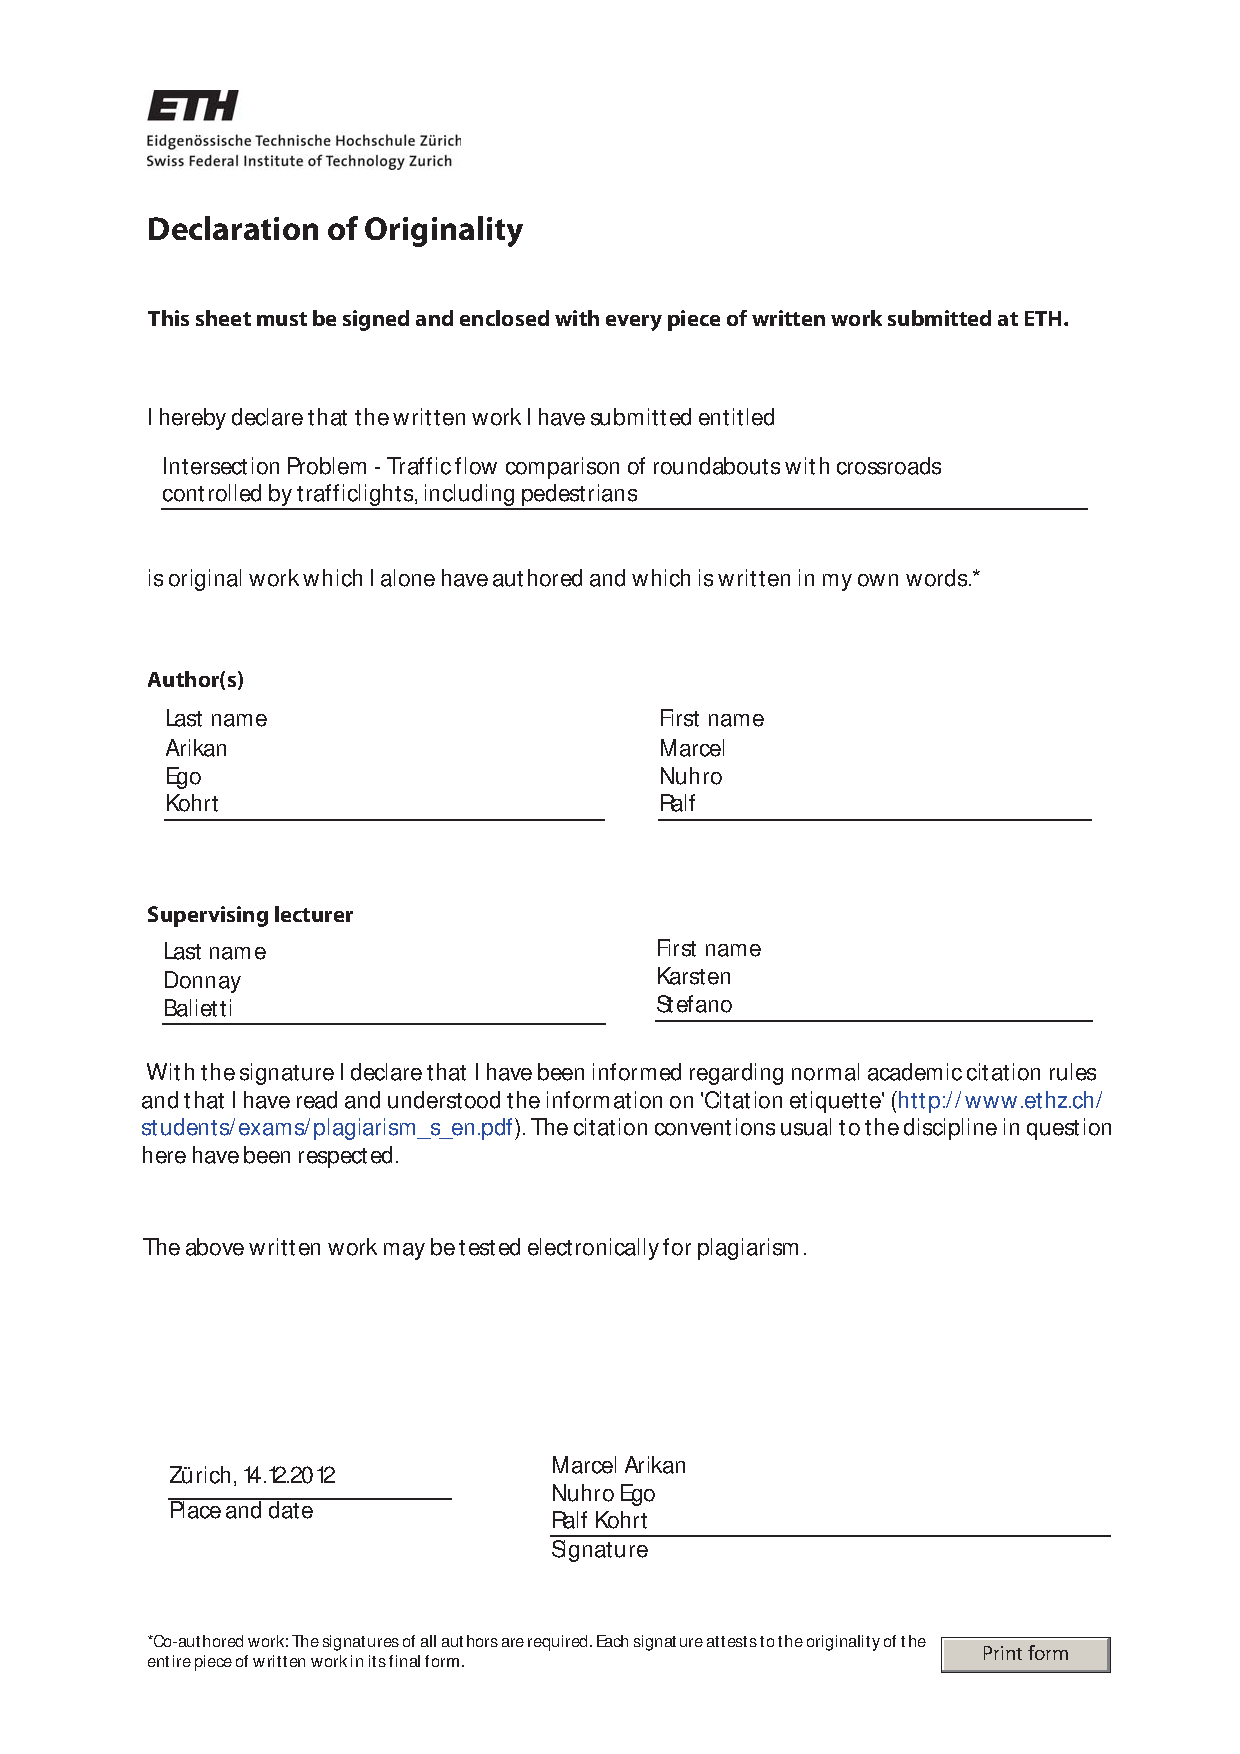
\includepdf[pages={1}]{confirmation_of_originality.pdf}

% IMPORTANT
% you MUST include the ETH declaration of originality here; it is available for download on the course website or at http://www.ethz.ch/faculty/exams/plagiarism/index_EN; it can be printed as pdf and should be filled out in handwriting
%%%%%%%%%% Table of content %%%%%%%%%%%%%%%%%

\tableofcontents

\newpage

%%%%%%%%%%%%%%%%%%%%%%%%%%%%%%%%%%%%%%%
\section{Abstract}
In our simulation, based on cellular automata, we have tried to compare roundabouts to crossroads, controlled by traffic lights, with respect to the traffic flow. We defined the traffic flow as the product of car density and average speed of the cars. Whereever reasonable, the Nagel-Schreckenberg model has been implemented. The main input parameters are car density and pedestrian density. There are three different signalisation modes of the trafficlight, depending on the pedestrian density. We expected roundabouts to be more efficient at low pedestrian densities for every car-density, but if pedestrian density rises the advantage should melt. Indeed, we have found, that the flow decreases approximately linearly to zero with the pedestrian-density rising after having reached the maximum in roundabouts. In contrast, the flow in crossroad is, as expected, rather low but never vanishes. 
\section{Individual contributions}
\section{Introduction and Motivations}
Several groups in this course have simulated roundabouts and crossroads before. Our work is a development of and in addition to �Traffic Dynamics�, written by Tony Wood and Bastian B�cheler in May 2010. In difference to their simulation we added pedestrians and implemented crossroads with lights instead of �priority to the right� organisation. They showed impressively, that roundabouts are much more efficient than crossroads, nearly independent of the car density. They have concluded, that �their model confirms, that the increase in popularity of roundabouts over the last years is justified�. In our view one important parameter was missing: the pedestrian density. As we have lived so far in cities, we have had occasions enough to observe that in the mornings and evenings some large roundabouts are just blocked, when pedestrians are allowed to cross the streets, especially when in the middle of the roundabout is a station for trams or buses. Depending on the pedestrian density we have implemented three different signalisation modes in the crossroads. For high pedestrian densities there won't be any conflicts between pedestrians and cars. So we thought that at least at this stage, crossroads may be in advantage to roundabouts. 
Some results
\section{Description of the Model and Implementation}

\subsection{Description of the main function}

In our model one can compare roundabouts with crossroads, controlled by traffic lights. One can use an arbitrary combination of roundabouts and crosslights in a $N \times M$ map.\\Main input of the simulation are car and pedestrian densities, which can be entered as arrays. The simulation can be done with different probabilities for the car to go straight ahead. Cars turning left or right will have the same probability. The simulation will generate a plot over these densities as x- and y- axis and the average flow and average speed as z-axis in different colors. 

\begin{center} 
$flow = density \cdot speed$
\end{center}

\subsubsection{Implementation}

We have created a big matrix to display the simulation, containig all roads and intersections. Cars will be painted in blue and pedestrians in yellow. To the right of lanes heading towards a crossroad and to the left of lanes for cars turning left are traffic light cells, which are red or green. Next to the lanes leaving is a traffic light too, but for pedestrians. Many matrices more are needed to store status informations that can change. So for most following matrices, there are two versions, representing current and next status. After every iteration status next will assigned to current. 

\subsection{crossroad}
Depending on the pedestrian density, there are three different signalisation modes. For densities smaller than 0.3, cars that turn can always be blocked currently by a pedestrian. If the density is between 0.3 and 0.6, they can only block cars turning left. And if the density is even higher there should be no conflicts between cars and pedestrians. But if the car densities are very high, it can happen that the fixed yellow phase for changing the signalisation is too short to let all the cars leave the crossroad.\\

A further input parameter in the main-function is the probability of a car driving straight ahead. Cars that turn left and right have the same probability. So depending on these probabilities the relative time for light phases are different. To get the absolute time of a phase, one has to multiply it with a constant, indicating how often you change the signalisation.\\

It would be efficient if cars leaving one intersection would just arrive at the next one in a �green�-phase, so that the crossroad could take advantage of the randomisation process when entering a roundabout. A clever solution for this interesting problem is left to a next group, hopefully. We just added a phase offset between two crossroads, defined by the average time a car needs to drive from one intersection to the next and the fixed street lengths.\\

In contrast to the simulation of Wood and B�cheler and to the roundabout, cars entering the crossroad can have speed bigger than one cell per iteration. So cars can drive straight ahead with maximal speed of 5 cells according to the Nagel-Schreckenberg model. Cars turning left or right are limited to maximal 2 cells per iteration.\\

\subsubsection{Implementation}
A crossroad consists of three $6 \times 6$-Matrices, so that for every cell information about is there a car, its speed and direction can be stored. Furthermore two $4 \times 8$ -Matrix for 4 lanes of length 8 cells at every street heading towards the crossroad for cars turning left are needed to decide if there's a car and store its speed. For cars driving ahead or turning right one $4 \times 8$-Matrix indicates the direction. 

\subsection{Roundabout}
Our implementation of the roundabout consits of a circle with 12 cells and 4 roads, which lead towards it. Every street has pedestrian crossings in front of each roundabout. 
Like in the real world, cars inside the roundabout have priority over cars wanting to enter them and pedestrians have priority over cars at the pedestrian crossings, 
with the addition, that pedestrians will only walk on the road if there is no car staying or driving on the cell they wants to walk on. 
Inside the crossroad the speed a car can have is limited to 1 cell per iteration step. \\

A car which wants to leave the roundabout at the next exit will indicate, in our plot this is shown by giving these cars a darker colour. 
The exit a car will take is calculated from the probability ahead like in the crossroad, but with a fixed probability of 5 \% for a car which will take the 4th exit (i.e. the car will turn around). \\
\subsubsection{Implementation}
This is implemented with many arrays, three arrays for the circle, one which shows whether there is a car or not, and if the car wants to leave at the next exit. 
The second is used to store the velocity of the car and the third is used to store, how many exits the car will pass without leaving.\\

The entries and exits of the roundabout are randomly blocked by pedestrians. For this reason two 'buckets' are created, representing pedestrian islands between inwards and outgoing streets. If a pedestrian crosses an outgoing street, the bucket makes sure, that in the next iteration inwards street will be blocked. 


\subsection{Graphical implementation}

One very important part in simulating a specific problem is visualization. First for checking if a given implementation makes sense the way one has written it, for bug fixing and for adjusting the parameters of the model to the real world problem.

\subsubsection{Preparatory work}
Before programming something out of the head one has to create an idea of how a problem could be implemented. One has to be careful to not exaggerate the model and fix too much on unimportant details, but to keep the main ideas clear and simple. 

\begin{figure}[htb]
	\centering
		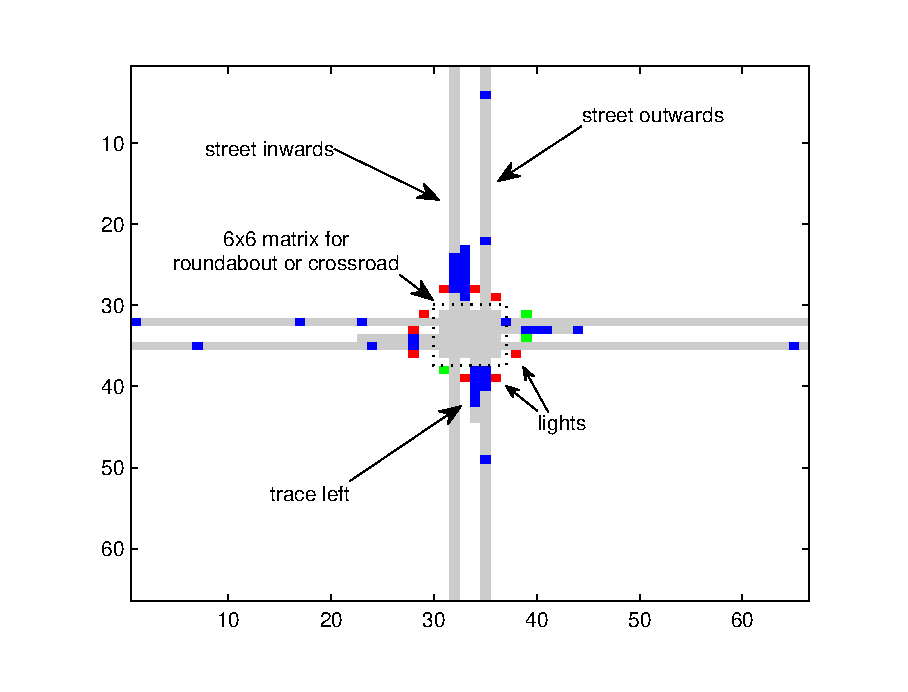
\includegraphics[width=0.8\textwidth]{images/description_mapping_overview.eps}
	\caption{Overview over the implementation of the plot.}
	\label{fig:description_mapping_overview}
\end{figure}

\autoref{fig:description_mapping_overview} shows how we finally ended in, because it shows the elementary cell of each intersection. Our model consisted of
\begin{itemize}
	\item a intersection (either roundabout or a crossroad)
	\item 8 streets for each direction of the crossroad (each with a out- and ingoing street)
	\item	pedestrians (not in the figure)
	\item	cars (in blue)
	\item	traffic lights for the cars and pedestrians in the case of a roundabout
	\item a trace for the cars that turn left in the case of a crossroad
\end{itemize}

In the following sections I will explain the programming details of this figure.

\subsubsection{Implementation}
For each type of intersections we have written a function that works out the paths of the cars and returns this information in a $6 \times 6$ matrix. Furthermore information about the pedestrians, the traffic light phases and the cars on the left trace are returned. I implemented these by creating a large matrix

\[
 \begin{split}
\mathrm{map} = (\mathrm{(No. \ of \ intersections \ in \ x \ direction)} \cdot (2 \cdot \mathrm{streetlength} + 6) \times \\ 
 \mathrm{(No. \ of \ intersections \ in \ y \ direction)} \cdot (2 \cdot \mathrm{streetlength} + 6))
\end{split}
\]

in which we wrote all elements listed up above for each time step, that we looked at. The elements of the maps were encoded in a color code from $0$ to $2$, i.e.
\begin{itemize}
	\item	Car = $0.6$
	\item	Red light = $1.6$
	\item	Pedestrian = $0.8$
\end{itemize}
that were written into this large matrix.
By plotting this matrix with
\begin{center}
\texttt{imagesc(map)}
\end{center}
and using a colormap we were able to create a relatively realistic model (see figure above).


\begin{figure}[htb]
	\centering
		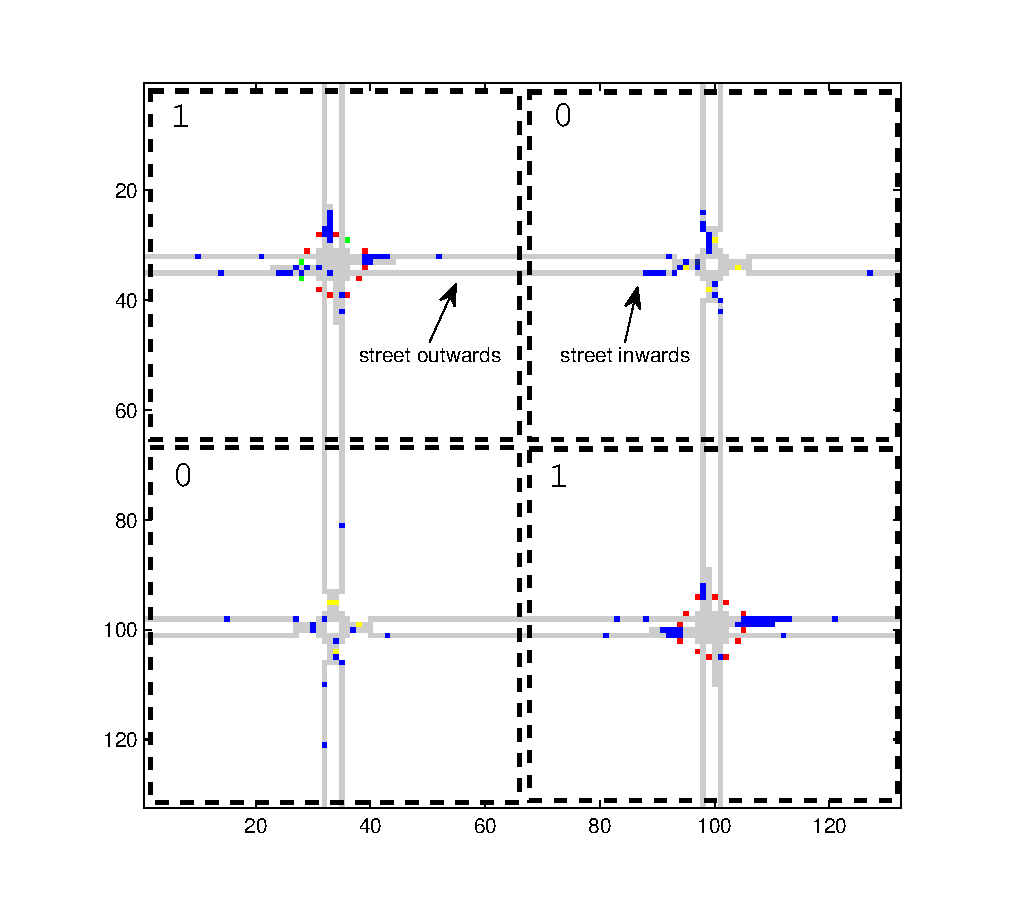
\includegraphics[width=0.8\textwidth]{images/description_mapping_detail.eps}
	\caption{Details about the implementation of the plot in the case of many intersections.}
	\label{fig:description_mapping_detail}
\end{figure}

We wanted to analyze how the traffic flow changes when we have many intersections in a map that are connected together to reproduce a more realistic view of the world. The configuration of each map was written into a matrix. This matrix had $0$ (corresponding to roundabout) and $1$ (corresponds to crossroad) as entries and corresponds to the rough structure of the map. Let's demonstrate this with \autoref{fig:description_mapping_detail}. We see in the top left and bottom right corners two crossroad and in the top right and bottom left corner two roundabouts. Naturally this would be denoted in a matrix as
\[
	\left(\begin{matrix}
1 & 0\\ 
0 & 1
\end{matrix}\right)
\]
and this is how we implemented it. Then the outgoing streets of the one cell are connected to the inwards streets of the neighboring cell and programing this, this results in these dynamic maps.

Furthermore we added the support of saving a video output of the this specific configuration. For further details see the code in the listings (see \autoref{plot_map}).

\newpage
\section{Execution and User Instructions}
\subsection{User Instructions}
The Simulation consists of total 14 functions. Our main-function to be executed is called traffic. 
The user will be asked, what city configuration he would like to simulate. The input has to be a $N \times M$-Matrix with entries 0=roundabout or 1=crossroad. 
Then car density, probability for car driving ahead and pedestrian density are numbers between 0 and 1. A density of 0 means no cars, whereas 1 means on every single cell except the ones in the intersections stays a car. 
Densities can be entered as arrays, so the simulation will run for every single entry. 
Afterwards the user can decide, whether he wants to display the simulation, if slow motion is required and if he wants to store the data average speed and average flow. \\
traffic.m will then load trafficloop.m, which will then call trafficsim.m. Our main loop for every iteration is there and In trafficsim. is our main loop for every simulation and here the output graphics, videos etc. will be created. 

\section{Simulation Results and Discussion}

{\centering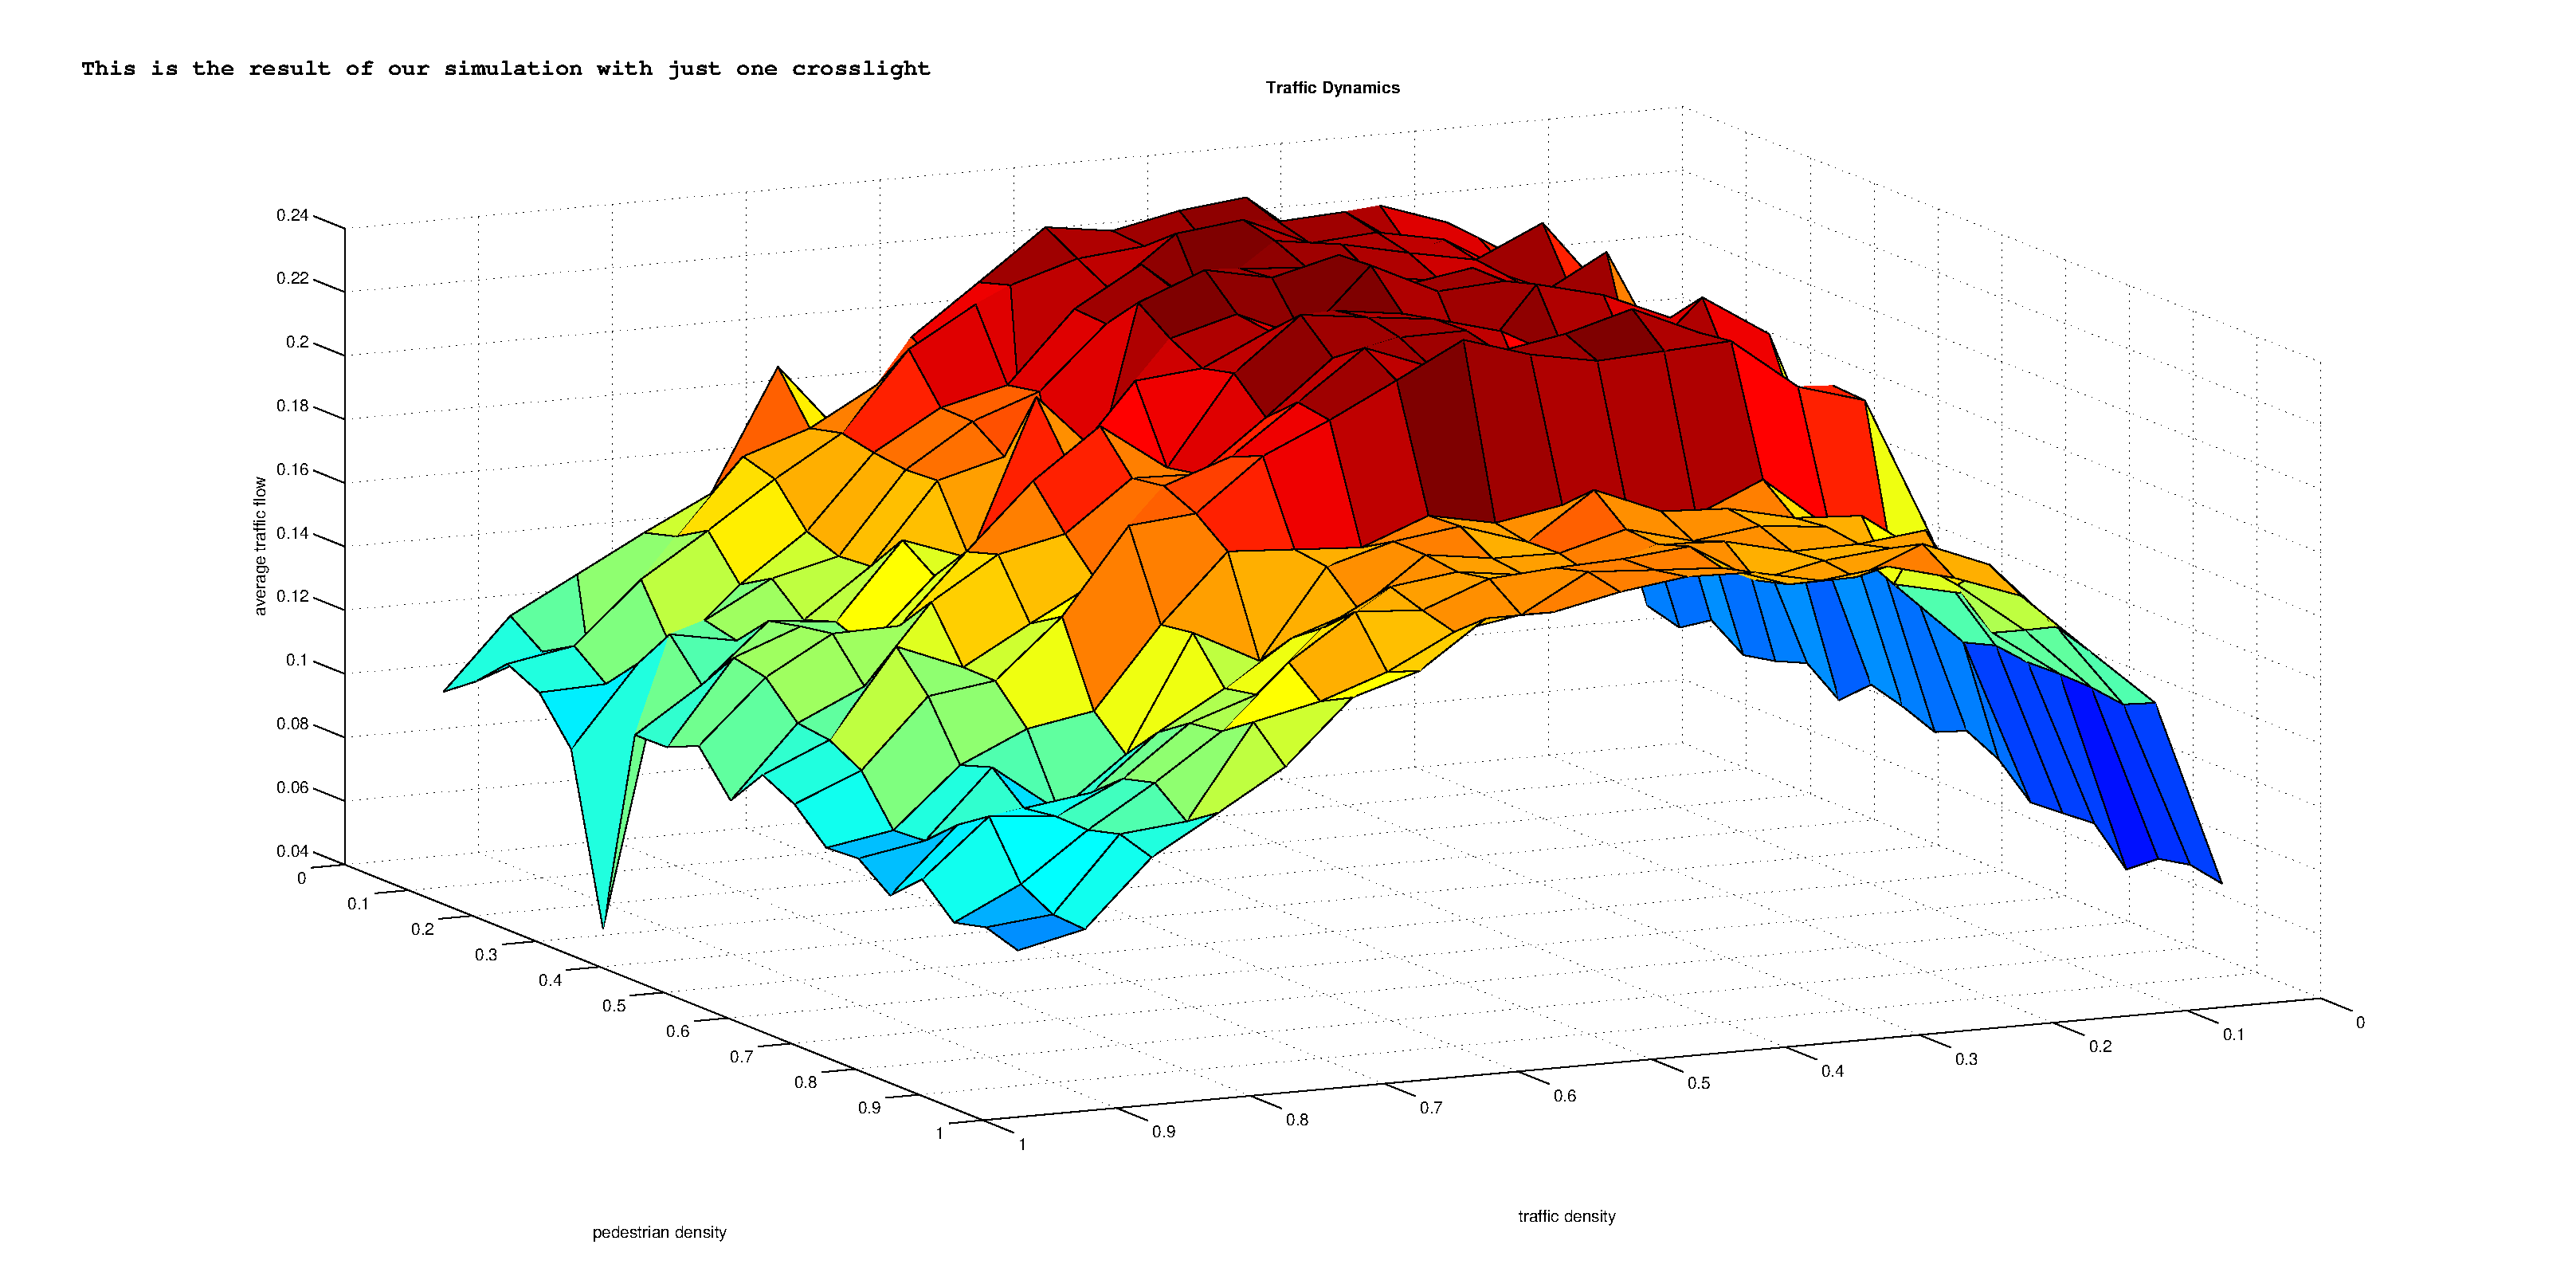
\includegraphics[width=15cm]{images/1-1-trafficlight.eps}

In this plot of one crosslight, one can clearly see the linear increase of traffic flow with increasing car density till ~0.25 after that it is more or less constant till it drops linearly at car densities higher than 0.6. 
One can also see that it does depend only weakly on the pedestrian density, but for high pedestrian densities above ~0.8 we see a small drop. (caused by a different traffic light mode)

{\centering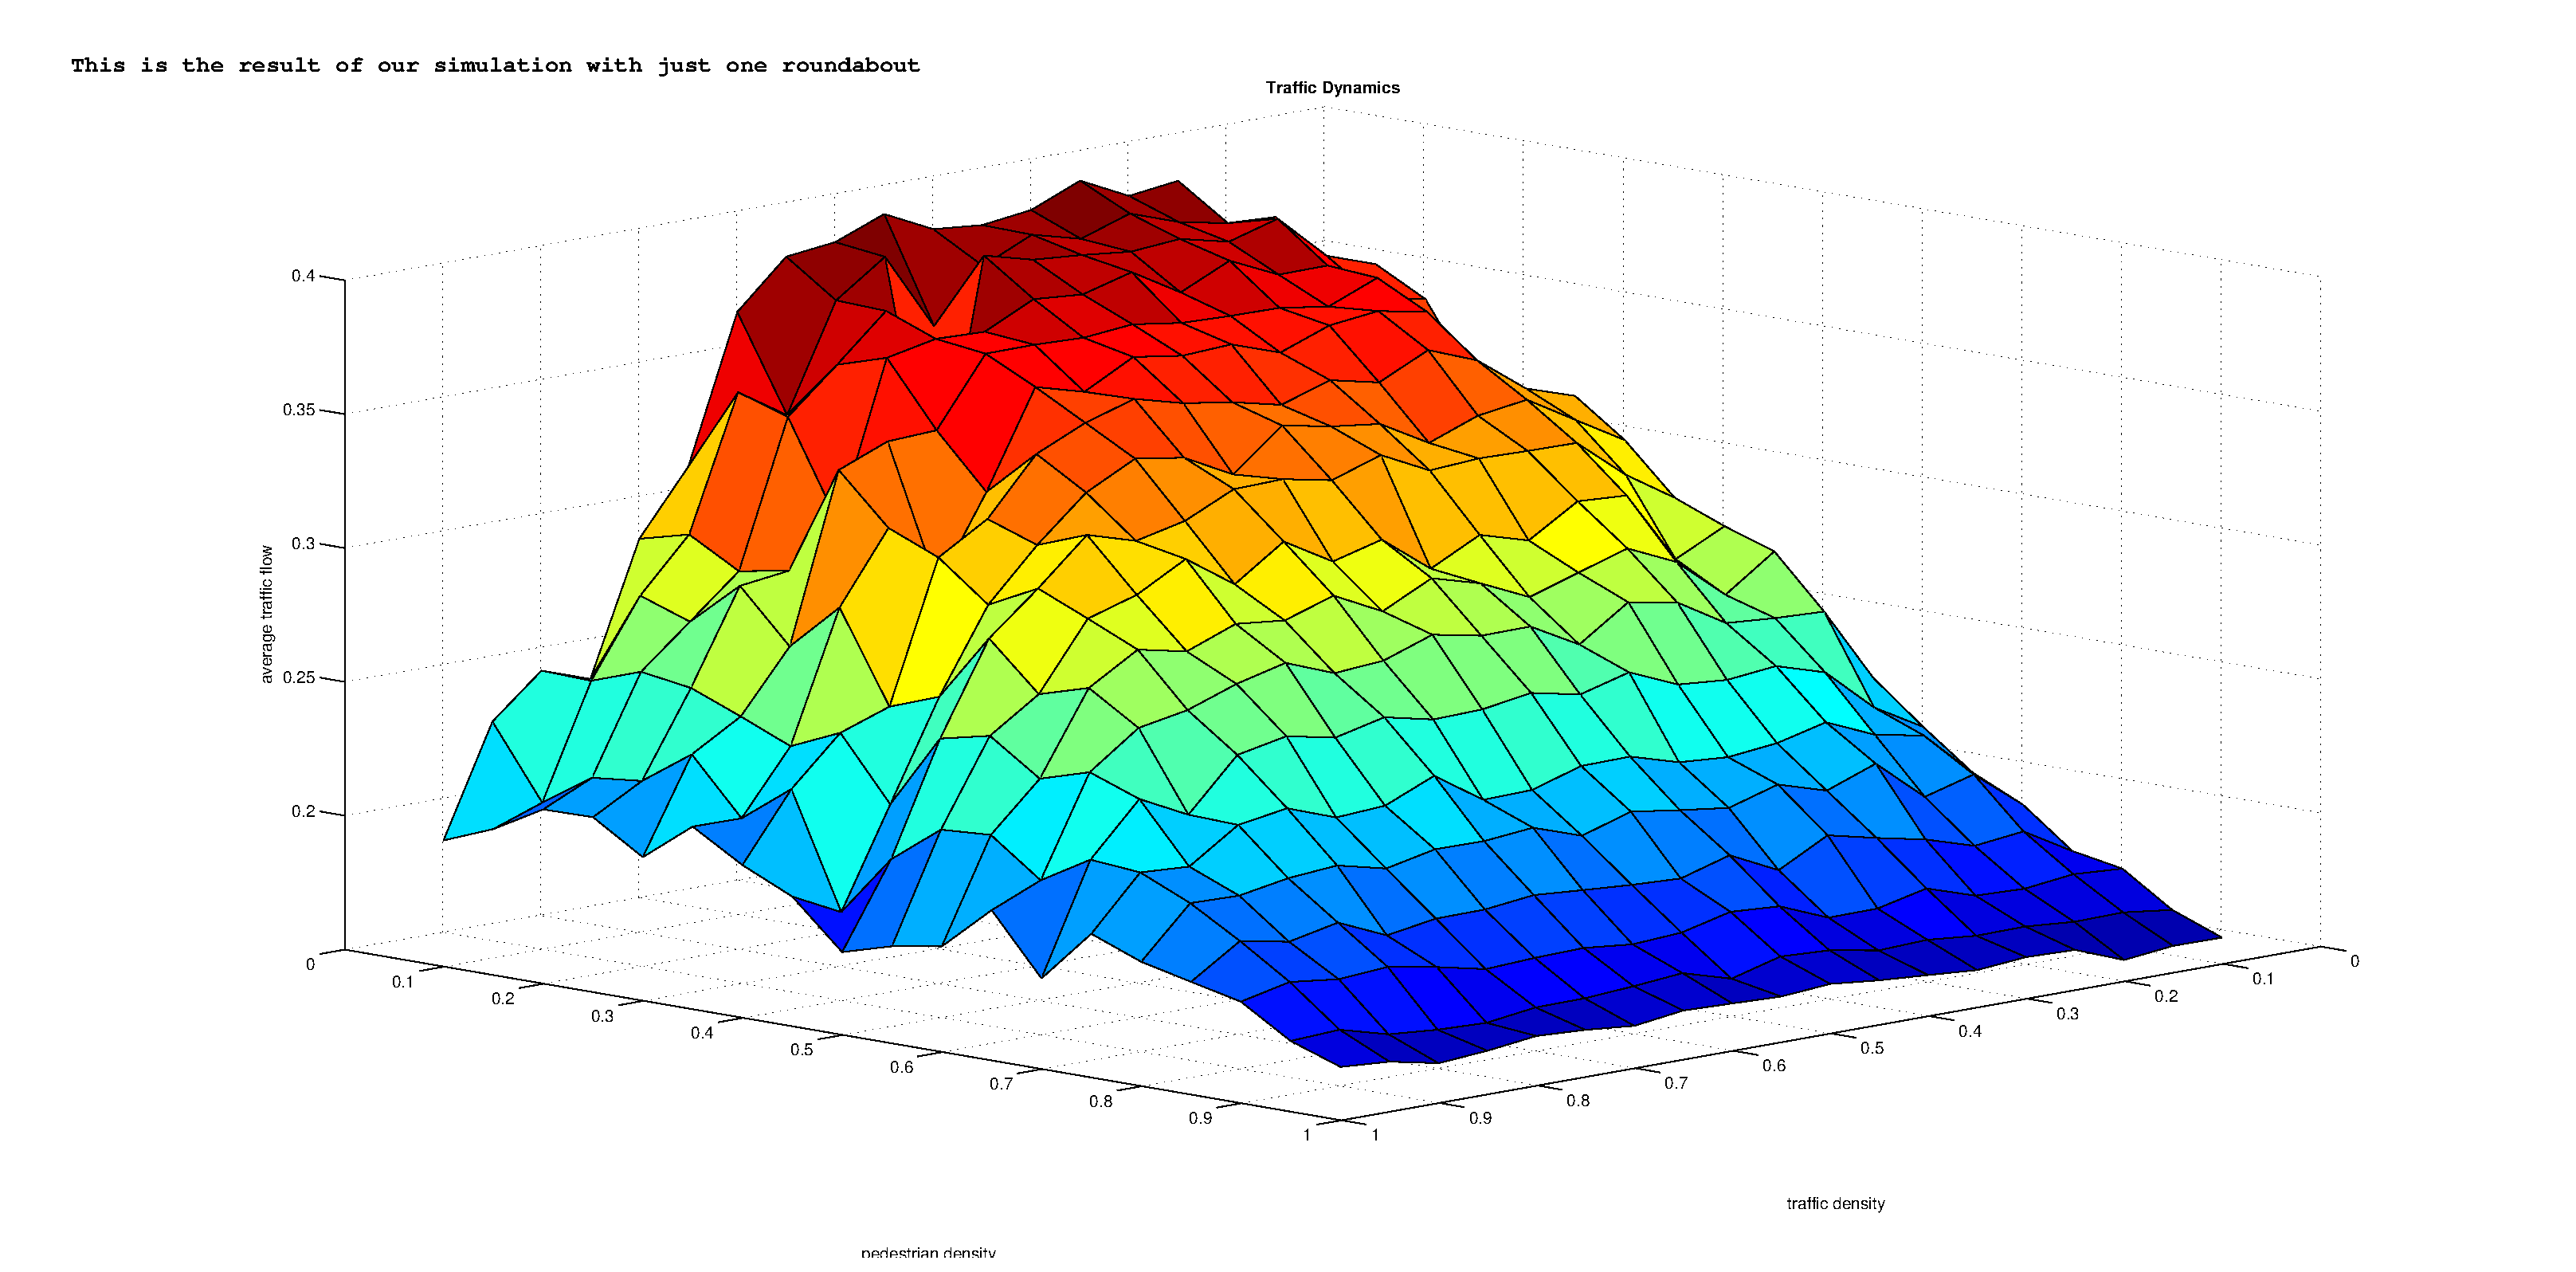
\includegraphics[width=15cm]{images/1-1-roundabout.eps}

In this plot of one roundabout the linear decrease in flow with increasing pedestrian density is clearly visible. And for a const. pedestrian density one sees also the expected result, 
which is a linear increase, then for some time a const flow and ending with a linear decrease for increasing car densities. Compared to the flow of one trafficlight one can see that a roundabout is much more efficient (almost twice the flow) for low pedestrian densities
and less efficient for low densities.

{\centering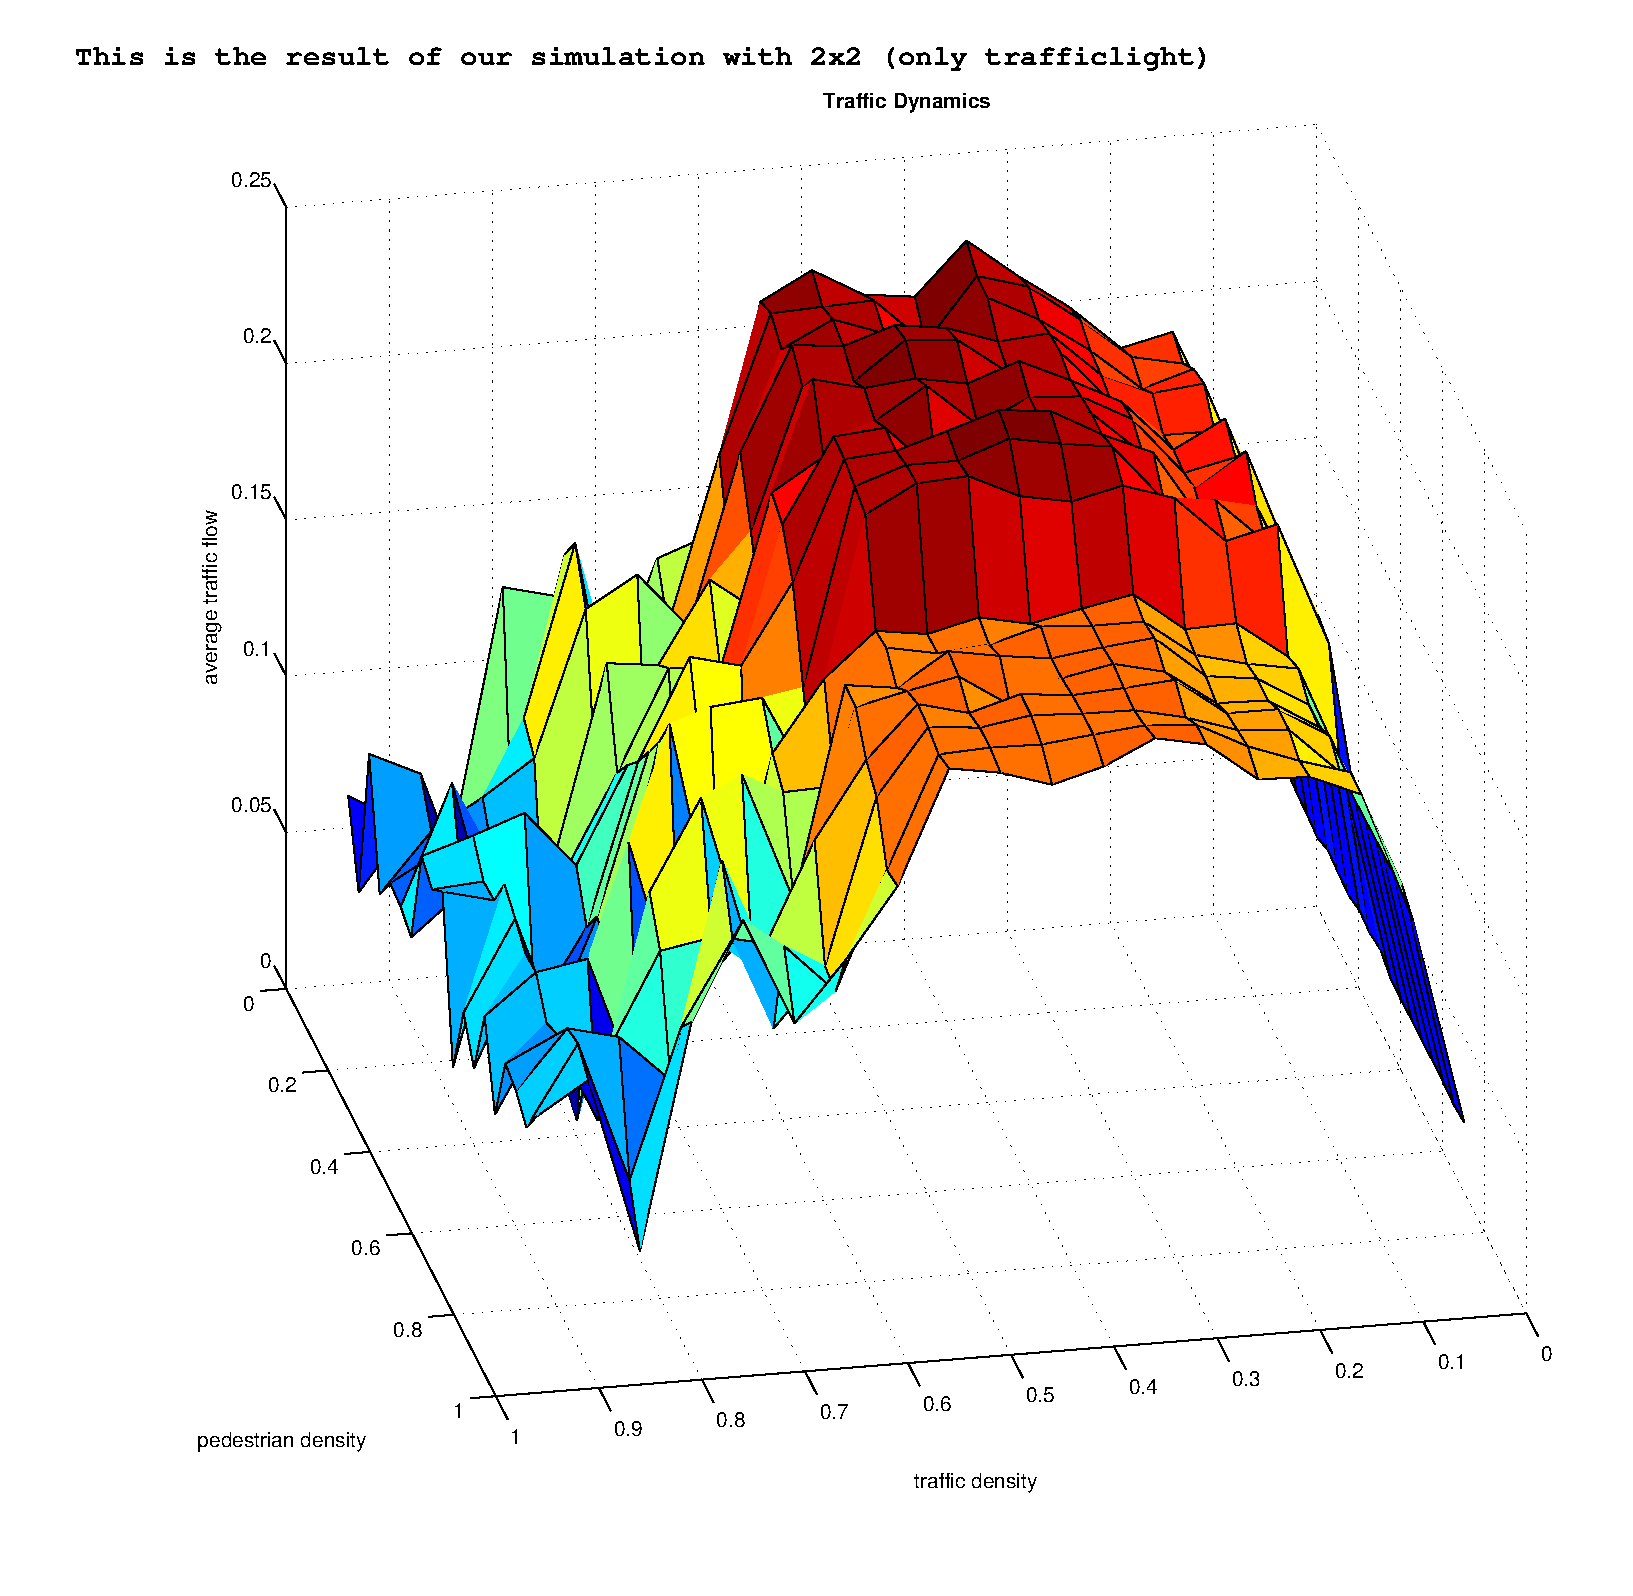
\includegraphics[width=15cm]{images/2-2-trafficlight.eps}

This result does not differ much from the result with just one trafficlight, but one can see that the linear in-/decrease has a higher slope.


{\centering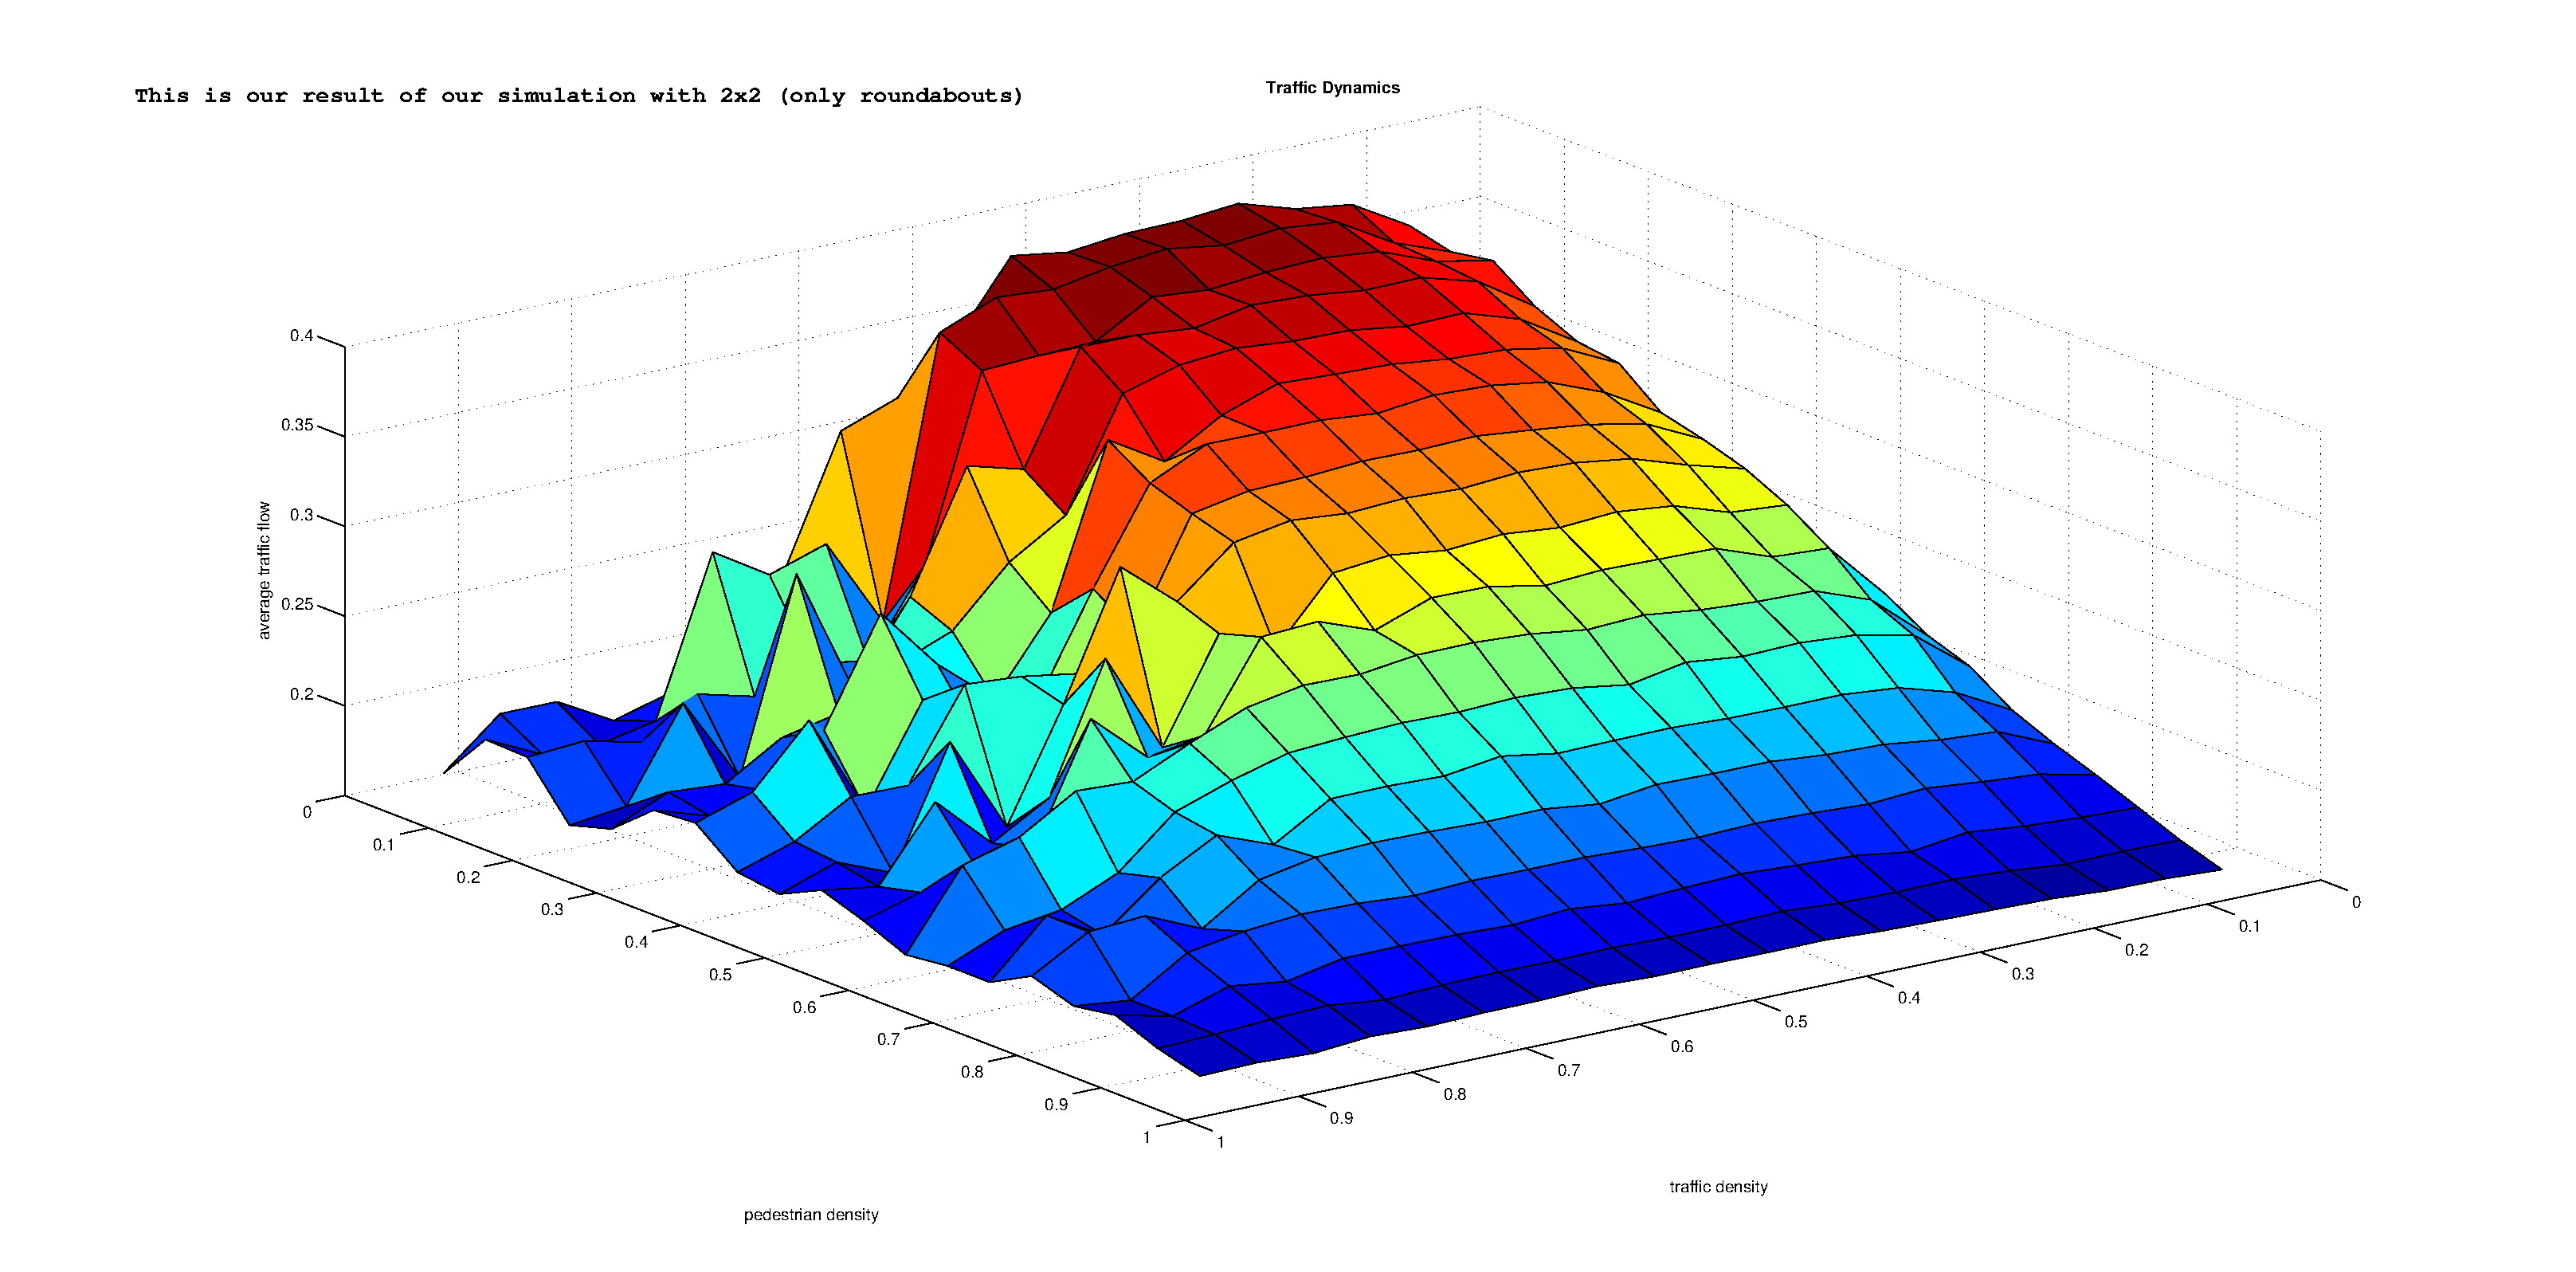
\includegraphics[width=15cm]{images/2-2-roundabout.eps}

This result does not differ much from the single roundabout either, but here the slope of the linear decrease with increasing pedestrian densities is smaller.

{\centering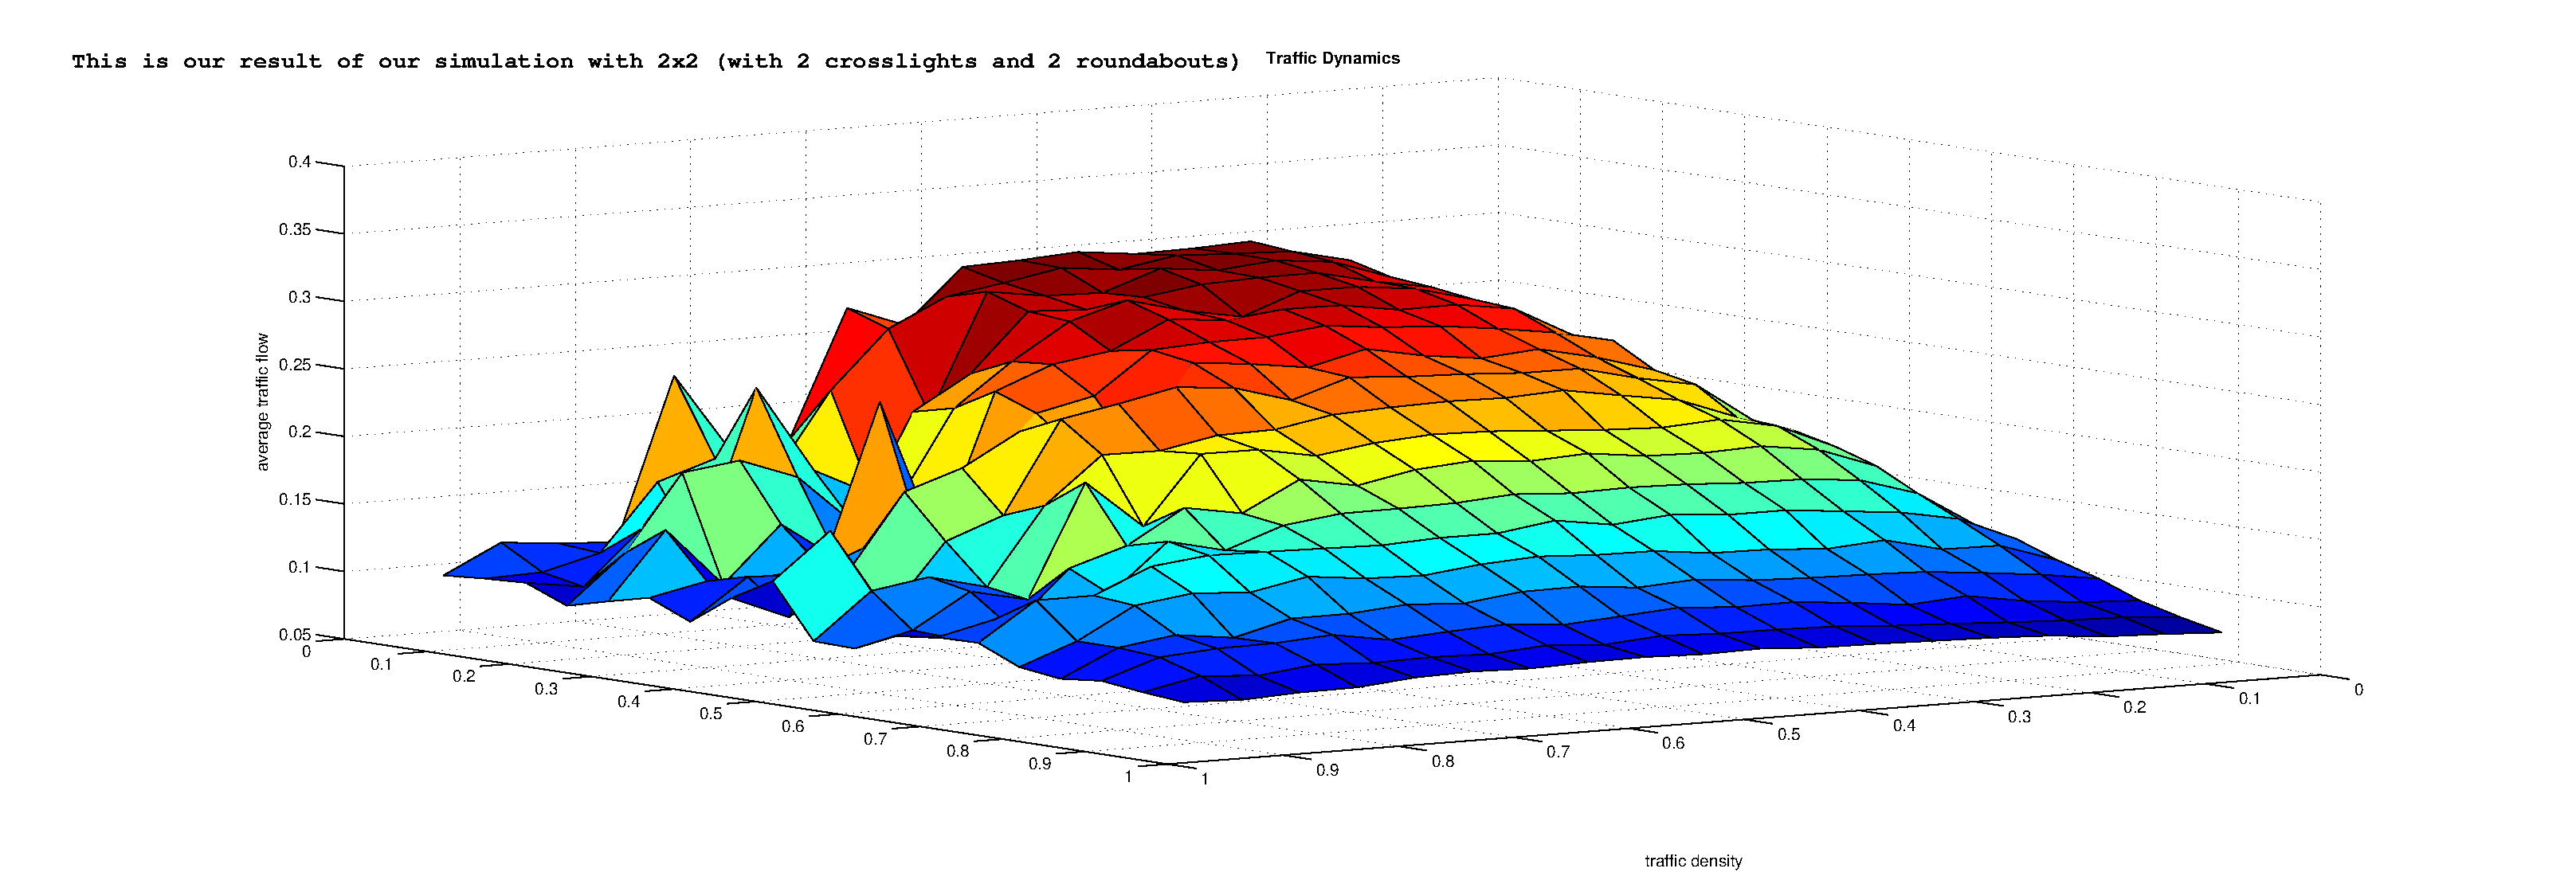
\includegraphics[width=15cm]{images/2-2-mix.eps}

In the combination case of both methods, the characteristic looks dominated by the roundabout (i.e. it does not look much different to the graph above) but here the flow rates are lower. With higher car dnsities random processes are getting more important
and thus the graph does not look so smooth anymore.

{\centering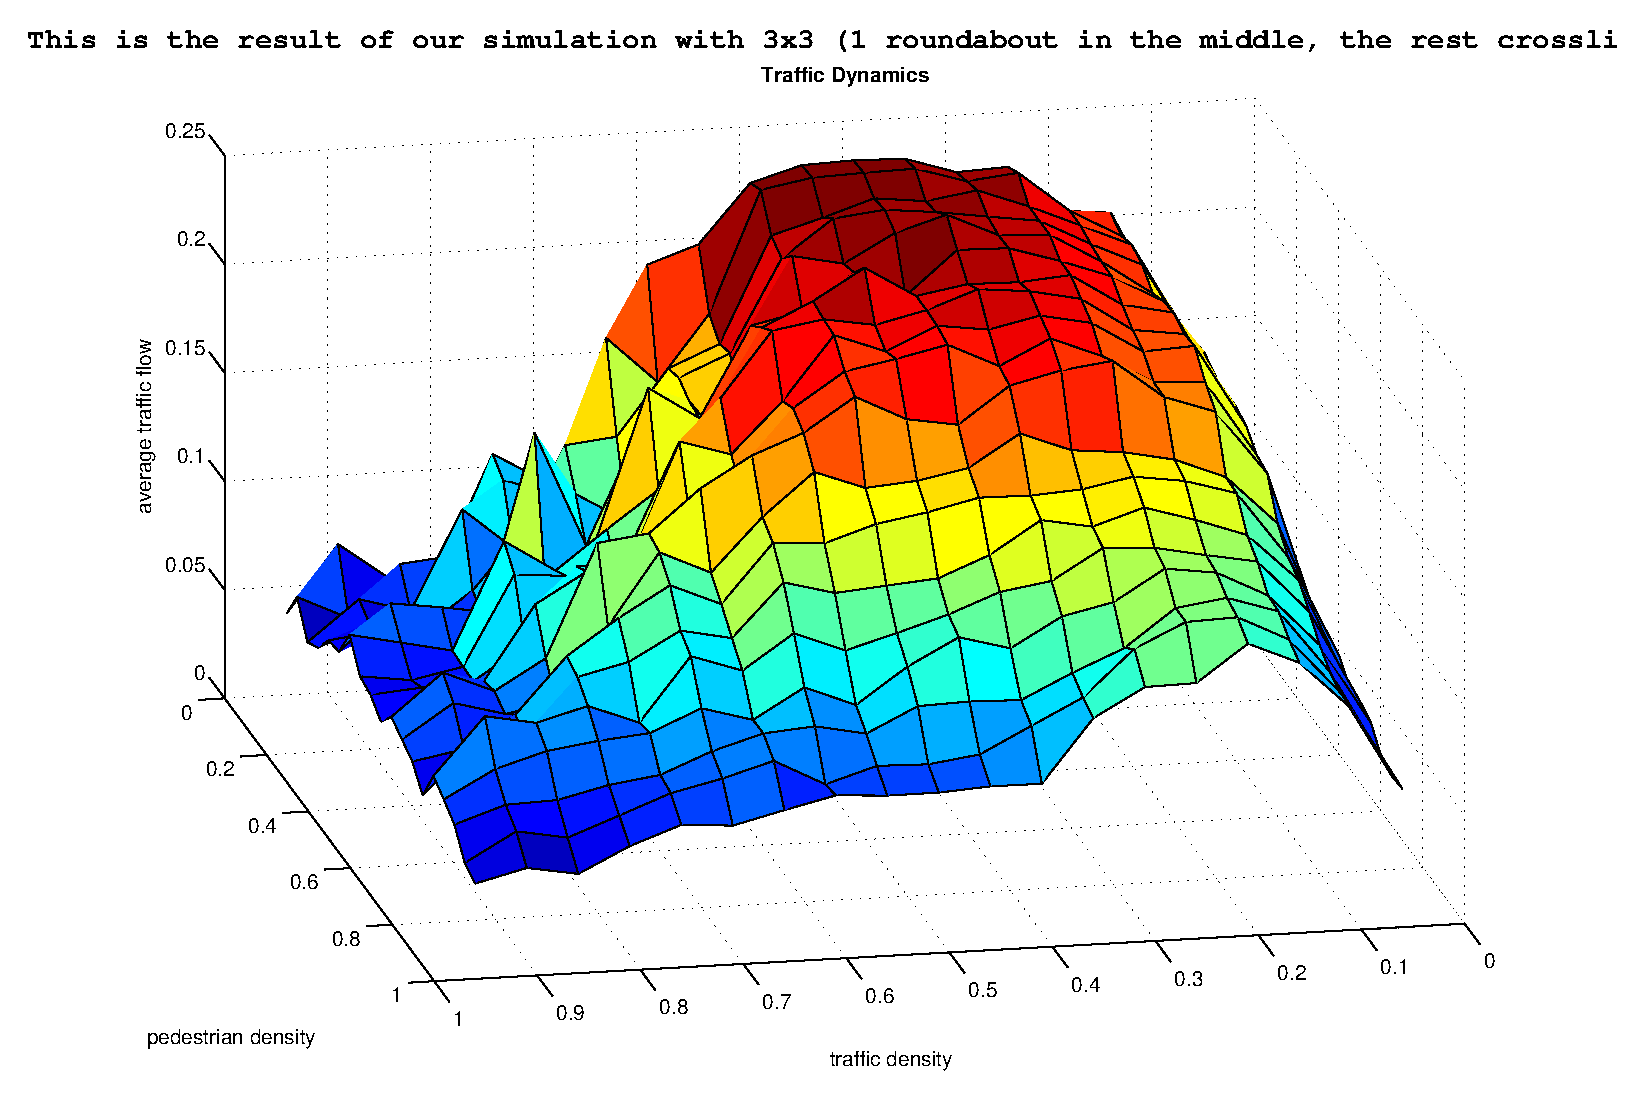
\includegraphics[width=15cm]{images/3-3-mix.eps}

Here it is visible, that just one roundabout in the middle is able to block for high pedestrian densities, were as for lower ones this is clearly dominated by the eight trafficlights.

\section{Summary and Outlook}

\appendix
\listoffigures

\clearpage
\section{Listings}
\label{sec:Listings}

\subsection{General Codes}


%\lstinputlisting[language=Python,caption={zoom.py},label=zoom]{listings/zoom.py}

\subsection{Matlab}
\label{subsec:Mathematica}

%\lstinputlisting[caption={asdfasdf},label=asdfasdf]{listings/blabla.nb}

\clearpage
\bibliographystyle{plain}
\bibliography{bib/references}


\end{document}  



 
